\begin{chapterfig}[Thesis]
\inputonce{figures/arch_style}
\label{cfig:thesis}
\setlength{\platformlayerwidth}{21ex}
\tikzset{
	chapter node/.style={anchor=mid east,font=\figureversion{text,tab}\itshape,outer xsep=1ex,outer ysep=0,inner sep=0},
	platform node/.style={outer sep=0,minimum width=10em},
	zoom/.style={draw=niceblack,densely dotted,thick,overlay},
	chapter shade/.style={draw=nicegray,dashed},
	software/.append style={platform node,layer fill,minimum height=1em},
	interface/.append style={platform node,model,minimum height=1em},
}

% set of layers
\platformlayer[padded]						(app)	{application};
\platformlayer[model,padded]				(pm)	{programming model};
\platformlayer[model,padded]				(moc)	{model of computation};
\platformlayerglue[padded]					(moccm)	{parallelization tool};
\platformlayer[model,padded]				(cm)	{concurrency model};
\platformlayerglue[padded]					(cmmm)	{\acs{OS}, \acl{RTS}};
\platformlayer[model,padded]				(mm)	{memory model};
\platformlayer[padded,minimum height=5em]	(hw)	{actual hardware};

% cross layers
\crosslayerright[]	<moc.north east->			()		{platform: \Starburst};
\crosslayerleft[]	<app.north west-mm.west>	() 		{software layers};
\crosslayerleft[]	<mm.west->					() 		{hardware};

% corresponding models in actual platform
\begin{pgfonlayer}{deepground}
	\platformlayersnode[interface]		<pm-moc>		+15ex () {C, C++, \lcalc};
	\platformlayersnode[interface]		<mm-mm>			+15ex () {\acs{PMC}};
	\platformlayersnode[interface]		<cm-cm>			+15ex (pthread) {};
	\begin{scope}[
			x=1em,y=1em,
			shift={(pthread.west)},
			thread/.style={software,no wrap text,no icon,minimum size=1em,font=\scriptsize,outer sep=.5\pgflinewidth,inner sep=0},
	]
		\node[thread,anchor=west] (t1) at (.6,0) {T};
		\node[thread,anchor=center] (t2) at ($(t1.center)+(1.5,0)$) {T};
		\node[thread,anchor=center,draw=none,fill=none,no shade] (tn) at ($(t2.center)+(1.2,0)$) {\rule[0pt]{0pt}{1.3ex}$\cdots$};
		\node[draw=none,fill=none,minimum size=0,anchor=mid west,outer sep=1ex] at (tn.east) {Pthreads};
%		\path[use as bounding box] (current bounding box.north east) rectangle (current bounding box.south west);
		\path[zoom] (t1) -- +(0,-1em);
		\path[zoom] (t2) -- +(0,-1em);
%		\path[zoom] (tn) -- +(0,-1em);
	\end{scope}
\end{pgfonlayer}

% corresponding software in actual platform
\platformlayersnode[software]		<app-app>		+15ex () {\SPLASH and \NoFib};
\platformlayersnode[software]		<moccm-moccm>	+15ex () {\ourfp};
\platformlayersnode[software]		<cmmm-cmmm>		+15ex (os) {\Helix};
\platformlayersnode[platform node]	<hw-hw>			+15ex (soc) {};
\begin{scope}[
		x=1em,y=1em,
		shift={(soc.center)},
		connection/.style={thick,draw},
		component/.append style={no wrap text,font=\scriptsize,minimum size=1.25em,inner sep=0},
		interconnect/.append style={minimum width=7em},
		memory/.append style={minimum width=5em},
	]
	\node[core,anchor=south] (p1) at (-3,1) {};
	\node[core,anchor=south] (p2) at (-1.5,1) {};
	\node[core,anchor=south] (p3) at (0,1) {};
	\node[core,anchor=south] (p4) at (1.5,1) {};
	\node[plain label,anchor=south] (pn) at (3,1) {\strut$\cdots$};
	\node[memory,anchor=north] (mem) at (0,-1) {\strut memory};
	\path[connection] (p1.south) -- +(0,-.5);
	\path[connection] (p2.south) -- +(0,-.5);
	\path[connection] (p3.south) -- +(0,-.5);
	\path[connection] (p4.south) -- +(0,-.5);
%	\path[connection] (pn.south) -- +(0,-.5);
	\path[connection] (mem.north) -- +(0,.5);
	\node[interconnect,anchor=center] (noc) at (0,0) {\strut interconnect};
	\path[zoom] (os.south west) -- (p2.north west);
	\path[zoom] (os.south east) -- (p2.north east);
\end{scope}

% corresponding chapters
\node[platform node,chapter node,anchor=south,minimum height=\platformlayerheight] (tr)	at (app.north)		{\strut trends};
\platformlayersnode[chapter node]	<tr-app>		+-2ex (c2)	{\Cref{c:starburst}};
\platformlayersnode[chapter node] 	<pm-moc>		+-2ex (c3) 	{\Cref{c:progmodel}};
\platformlayersnode[chapter node] 	<moccm-cm>		+-2ex (c6) 	{\Cref{c:concurrency}};
\platformlayersnode[chapter node] 	<cmmm-mm>		+-2ex (c5) 	{\Cref{c:memory}};
\platformlayersnode[chapter node] 	<hw-hw>			+-2ex (c4) 	{\Cref{c:hardware}};
\node[chapter node,anchor=south west,minimum height=\platformlayerheight]	at (c2.north west)	{\strut\Cref{c:introduction}};
\node[chapter node,anchor=south,minimum height=\platformlayerheight]		at (tr.north)		{\strut introduction};
\node[chapter node,anchor=north west,minimum height=\platformlayerheight]	at (c4.south west)	{\strut\Cref{c:conclusion}};
\node[chapter node,anchor=north,minimum height=\platformlayerheight]		at (hw.south)		{\strut conclusion};

% horizontal lines between all layers
\begin{pgfonlayer}{background}
	\path[chapter shade] (c2.north west) -- +(.99\linewidth,0);
	\path[chapter shade] (c3.north west) -- +(.99\linewidth,0);
	\path[chapter shade] (c4.north west) -- +(.99\linewidth,0);
	\path[chapter shade] (c5.north west) -- +(.99\linewidth,0);
	\path[chapter shade] (c6.north west) -- +(.99\linewidth,0);
	\path[chapter shade] (c4.south west) -- +(.99\linewidth,0);
\end{pgfonlayer}

\end{chapterfig}%


\setaachaptext[50]{the chapter with many-core trends and \Starburst}
\chapter{Trends in Many-Core Architectures}
\label{c:trends}
\label{c:starburst}

\begin{abstract}%
Based on a comparison of ten contemporary commercial many-core architectures, several trends can be observed.
The cores are relatively simple, and memory bandwidth per core is limited.
Most architectures have \aclp{MLC}, which are hardware cache coherent.
However, weak memory models are used.
In contrast to the attention in research, only a few architectures have \aclp{SPM}.
Our many-core architecture, \Starburst, captures both commercial and research trends.
\end{abstract}

\Cref{c:introduction} discussed the trends of microprocessors, and concluded that every processor will become a multicore one.
The tendency is that locality is crucial for performance.
In this chapter, we discuss several commercial processors in more detail, and relate these to the high-level trends above.
For evaluation purposes throughout the thesis, we designed and built the many-core system \Starburst*, which reflects these trends in current and expected future architectures.

\section{Ten many-core architectures}
\label{s:trends:architectures}

\Vref{t:trends:architectures} lists several \ix{multicore architectures} of the last several years.
These architectures all are single chip packages, deliver a high performance by utilizing multiple cores, and are commercially available, except for the experimental \IntelSCC.
All architectures are targeting high-performance computing, except for the Adapteva \Epiphany and Samsung \Exynos.
These two systems are designed for embedded systems with a limited power budget, like smartphones and tablets.

\ctable[caption={Architectures},label=t:trends:architectures]{
	>{\figureversion{text}}l
	>{\hspace{-2ex}}c
	>{\hspace{-.5ex}}r
	>{\hspace{-.5ex}\figureversion{text}}l
	>{\hspace{-1ex}}S[table-format=2.0]>{\hspace{-2ex}}r
	>{\hspace{-1ex}}S[table-format=6.0]}{}{
\FL							& [ref.]					& \hdr{year}	& \hdr{core type}
	& \multicolumn{2}{c}{\hdr[10ex]{cores (threads)}}
	& \hdr[10ex]{clock (\si{\mega\hertz})}	\ML
%Intel Pentium 4 531		&							& 2004	& Prescott, \xSixtyFour	& 1		& (2)	& 2993	\NN
%Sun Ultra\noac{SPARC} T2	& \cite{shah:ultrasparc_t2} & 2007	& \noac{SPARC} V9		& 8		& (64)	& 1165	\NN
\TILEGx						& \cite{tilegx}				& 2009	& \acs{DSP}				& 72	&		& 1000	\NN
\POWERseven					& \cite{kalla:power7}		& 2010	& C1					& 8		& (32)	& 3550	\NN
Oracle \UltraSPARC			& \cite{shin:ultrasparc_t3}	& 2010	& \noac{SPARC} V9		& 16	& (128)	& 1649	\NN
\IntelSCC					& \cite{howard:intel_scc}	& 2010	& Pentium-100			& 48	&		& 1000	\NN
\Inteliseven				& \cite{intel:3930k}		& 2011	& Sandy Bridge-E		& 6		& (12)	& 3200	\NN
Cavium \OCTEON				& \cite{cavium}				& 2011	& \noac{cnMIPS64} v2	& 32	&		& 1500	\NN
Adapteva \Epiphany			& \cite{epiphany}			& 2011	& \acs{RISC}			& 64	&		& 800	\NN
Samsung \Exynos				& \cite{yang:exynos}		& 2012	& \noac{ARM} Cortex-A9	& 4		&		& 1400	\NN
\Freescale					& \cite{freescale}			& 2012	& Power e6500			& 12	& (24)	& 1800	\NN
\XeonPhi					& \cite{intel:xeon_phi}		& 2012	& \xSixtyFour, vector	& 61	& (244)	& 1238	\NN
\Starburst					&							&		& \MicroBlaze			& 32	&		& 100	\LL
}

The table shows the number of cores and the total number of hardware-supported threads.
All these cores are homogeneous.
Although some systems include several accelerators, these are not taken into account for the core count.
As the number of transistors per chip increases, it is expected~\cite{borkar:future} that processors will integrate more heterogeneous cores or more accelerators, but this is not reflected in most of the systems listed---only the Cavium \OCTEON, \Freescale, and \Exynos integrate accelerators for graphics or other applications.
\Starburst*\footnote{Refer to \cref{a:etymology} for a description where the name comes from.} (in the form it is discussed in this thesis) is a homogeneous \MicroBlaze* system with a configurable core count of up to 32.
In contrast to all other architectures, it is mapped onto an \ac{FPGA}, which limits the clock frequency to \SI{100}{\mega\hertz}.

It is clear that contemporary high-end systems already require tens to hundreds of concurrent threads to utilize the full hardware of a single processor.
We do not consider (general-purpose) \acp{GPU} at this point.
Although these processors have thousands of cores, there usability is limited to parallel vector operations, like graphics and specific scientific workloads.
Moreover, there are constraints in memory accesses, code and data size, \etc.
In general, all systems of \vref{t:trends:architectures} are (supposed to be) programmed in C with threads, which cannot be done on a \ac{GPU}.

The setup of these systems is very common: cores have a small L1 instruction and data cache.
Often, cores are grouped in clusters of two or four cores, which connect via a low-latency interconnect to a shared L2 cache.
Furthermore, the individual cores or clusters are connected via a \ac{NoC} with a mesh topology or a multilayer bus to each other, and via one or more memory controllers to external \ac{DDR} memory.
The individual properties are discussed in more detail in the subsequent sections.


\section{Simpler cores, more performance}

Single-core processors use the increasing amount of transistors to implement complex microarchitectural features like out-of-order execution, exploiting \ac{ILP}, and deep pipelines.
These features are relatively costly, compared to the gained speedup~\cite{borkar:future}.
Once the burden to multicore and concurrency is overcome, it can be cost-effective to use simpler cores, but implement more of them.
For example, \XeonPhi's philosophy is to have many, but smaller cores than other Xeon processors.
The \UltraSPARC uses simpler in-order cores, but interleave instructions of many threads per core, such that the core's pipeline is filled, even when threads stall on cache misses, for example.
\Epiphany and \Exynos use \ac{RISC} cores to reduce power usage.
Interestingly, all systems either support \ac{SIMD} instructions or have specific accelerators.

\ctable[label=t:trends:core,caption={Core and memory performance}]{
	>{\figureversion{text}}l
	>{\hspace{-1ex}}S[table-format=6.0,table-auto-round]
	>{\hspace{-0ex}}S[table-format=3.2,table-auto-round]
	>{\hspace{-0ex}}S[table-format=2.3]
	>{\hspace{-0ex}}S[table-format=1.2,table-auto-round]
	>{\hspace{-0ex}}S[table-format=1.3,table-auto-round]
	}{
	\tnote[a]{Peak core--shared-memory bandwidth, based on the memory controller or the interface to the interconnect}
	}{
\FL						& \raisebox{-1.2em}[0pt][0pt]{\hspace{-1ex}\hdr[10ex]{\CoreMark* score \cite{coremark}}}
						& \raisebox{-1.2em}[0pt][0pt]{\hdr[10ex]{\CoreMark per \si{\mega\hertz}}}
						& \multicolumn{3}{c}{\hdr{shared-memory bandwidth\tmark[a]}}
						\NN
						& 
						& 
						& \hdr[8ex]{in total (\si{\giga\byte\per\second})} 
						& \hdr[10ex]{per core (\si{\byte\per cycle})} 
						& \hdr[13ex]{per \CoreMark (\si{\mega\byte\per\second})}
						\ML
%Pentium 4 531			& 5007.06			& 1.67			& 5.96		& 2.138 & 1.219 	\NN
%Ultra\noac{SPARC} T2	& 15298.36			& 13.13			& 42.7		& 4.916	& 2.858		\NN
\TILEGx					& 230195.61			& 230.19		& 53.6		& 0.80	& 0.238		\NN
\POWERseven				& 336196.25			& 94.70			& 95.4		& 3.605 & 0.291 	\NN
\UltraSPARC				& 87054.10			& 52.79			& 23.8		& 1.941	& 0.280		\NN
\IntelSCC				& 102240			& 102.24		& 21		& 0.44	& 0.210		\NN
\Inteliseven			& 150962.39			& 41.17			& 47.7		& 2.667	& 0.323		\NN
\OCTEON					& 153477.22			& 102.32		& 46.6		& 1.042 & 0.311		\NN
\Epiphany				& 78748.80			& 98.44			& 6.4		& 0.134	& 0.083 	\NN
\Exynos					& 22243				& 15.89			& 6.4		& 1.227	& 0.295		\NN
\Freescale				& 187873.61			& 104.37		& 46.9		& 2.333	& 0.256		\NN
\Starburst				& 4521				& 45.21			& .391		& 0.131	& 0.088		\LL
}

\Vref{t:trends:core} compares the processors' performance\footnote{Unfortunately, there is no \CoreMark score available for the \XeonPhi.}.
The \CoreMark*~\cite{coremark} benchmark is used to indicate the combined performance of all cores.
The benchmark tests integer and control flow performance, and minimizes the aspects of synchronization and memory bandwidth.
The \CoreMark score greatly differs between platforms.
However, when the score is compensated for the difference in clock frequency, it suggests that the systems with more cores perform better.
In this comparison, \TILEGx and \Freescale perform best, \Exynos and \Inteliseven worst.
So, many-core systems seem to perform well, and are therefore a promising computing platform.

Following this trend, \Starburst uses the simple resource-efficient \MicroBlaze* cores.
The \MicroBlaze is an in-order processor, and it is configured with a direct-mapped \SI{16}{\Kilo\byte} instruction cache and \SI{8}{\Kilo\byte} incoherent write-back data cache with a cache line size of 8~words, hardware multiplier, barrel shifter, and single-precision floating-point unit.
In this configuration, \Starburst's \CoreMark score per \si{\mega\hertz} is reasonable, but still below average.
However, with a score of \num{4521}, it is close to the single-thread performance of a Pentium~4 531 at \SI{3}{\giga\hertz}, which is listed with a score of \num{5007}~\cite{coremark}.

The peak bandwidth between the cores and shared off-chip \ac{DDR} memory is also listed in \vref{t:trends:core}.
The table lists the total bandwidth to all memory banks, the available memory bandwidth per core per clock cycle, and the bandwidth per \CoreMark unit.
Although the actual performance also depends on the rest of the memory hierarchy, these bandwidth numbers indicate a trend.
\TILEGx, \IntelSCC, and \Epiphany have the lowest bandwidth per core per clock cycle, but have the highest core count.
So, with increasing number of cores, the available bandwidth per core is reduced.
This is the same for the bandwidth per \CoreMark unit.
However, the numbers are closer together, which suggests that the relatively simpler cores result in a lower \CoreMark per core, and this compensates the reduction in available bandwidth.

Regarding the memory bandwidth, \Starburst is equivalent to \Epiphany.
However, compared to other architectures, the effects of the \ix{memory bottleneck} will be somewhat magnified in experiments with \Starburst.

\section{Transparent processing tiles}

%\ctable[caption={Processing tile properties}]{
%	>{\figureversion{text}}l
%	S[table-format=2.0,table-auto-round]
%	S[table-format=2.0,table-auto-round]
%	S[table-format=3.0,table-auto-round]
%	c}{}{
%\FL						& \hdr[12ex]{L1 I-cache size (\si{\Kilo\byte})}	
%						& \hdr[12ex]{L1 D-cache size (\si{\Kilo\byte})}	
%						& \hdr[10ex]{\acs{SPM} size (\si{\Kilo\byte})}
%						& \hdr[10ex]{explicit message-passing}	\ML
%%Pentium 4 531			&		&		&		&				\NN
%%Ultra\noac{SPARC} T2	& 		&		& 		&				\NN
%\TILEGx 				& 32	& 32	&		&				\NN
%\POWERseven 			& 32	& 32	&		& 				\NN
%\UltraSPARC 			& 8		& 16	&		& 				\NN
%\IntelSCC				& 16	& 16	& 16	& $\checkmark$ 	\NN
%\Inteliseven			& 32	& 32	&		&				\NN
%\OCTEON 				& 37	& 32	&		&				\NN
%\Epiphany				&		&		& 32 	&				\NN
%\Exynos 				& 32	& 32	& 128 	& 				\NN
%\Freescale				& 32	& 32	&		& 				\NN
%\XeonPhi				& ?		& ?		&		&				\NN
%\Starburst				& 16	& 8		& 4		& $\checkmark$ 	\LL
%}

Most architectures are shared-memory machines with multi-level \ix[cache]{caches}.
The hierarchy of cores and clusters is hidden behind a global address map and hardware cache coherency.
This setup has several drawbacks.

The behavior of caches is unpredictable at run time~\cite{blake:multiproc_survey}.
Whether a cache hit or miss occurs, depends on the cache contents, which are dynamically loaded, reconciled, and flushed.
A \acix{SPM} is a local memory next to the core, and is fully under software control.
As a result, \acp{SPM} are predictable~\cite{suhendra:spm}.
Moreover, they often give a higher performance, lower energy consumption, and lower hardware costs~\cite{nguyen:spm}.
Therefore, \acp{SPM} are an attractive alternative to caches.
However, only \IntelSCC and \Epiphany have a \SI{16}{\Kilo\byte} and \SI{32}{\Kilo\byte} \ac{SPM} per core, respectively.
Optimal \ac{SPM} allocation requires compile-time analysis of the application and efficient run-time control, which are both complex~\cite{blake:multiproc_survey}, or require a different programming approach.

\Starburst supports both setups: the \MicroBlaze caches the background memory, and also has a local memory, which can be used as an \ac{SPM}, but can also be accessed by other cores.
The architecture of one \MicroBlaze tile is depicted in \vref{fig:starburst:tile}.
The private \SI{4}{\Kilo\byte} \ac{RAM} contains the boot code, information about the system topology, and several kernel-specific data structures.
The \SI{4}{\Kilo\byte} \ac{SPM} is a dual port \ac{SRAM} that can be written by other \MicroBlazes.
Although this memory is generic, it can be used to implement core-to-core communication, such that only local memory is polled.
The \ac{LMB} allows single-cycle access to these memories.

\begin{figure}%
\inputfig{figures/starburst_tile}%
\caption{A processing tile of \Starburst. Arrows indicate master--slave relation.}%
\label{fig:starburst:tile}%
\end{figure}

The tile also contains an interrupt timer, which is used by the \ac{OS} for context switching.
This timer is the only interrupt source of the \MicroBlaze*.
The statistics counters track microarchitectural events, including the number of executed instructions, cache hits and misses, and stall cycles.
Because of resource constraints in the \ac{FPGA}, only one \MicroBlaze has these counters.


\section{Interconnect: coherency traffic \texorpdfstring{\protect\vs}{vs.} data packets}
\label{s:trends:noc}

%\ctable[caption={Shared memory bandwidth}]{
%	>{\figureversion{text}}l
%	S[table-format=4.0]>{\hspace{-2ex}}c>{\hspace{-2ex}}S[table-format=2.2]
%	S[table-format=2.3]
%	S[table-format=1.2,table-auto-round]
%	S[table-format=1.3,table-auto-round]}{
%	\tnote[a]{Peak core--shared-memory bandwidth, based on the memory controller or the interface to the interconnect}
%	}{
%\FL						
%						& \multicolumn{3}{c}{\hdr[10ex]{L1 I/D-cache (\si{\Kilo\byte})}} 
%						& \hdr[12ex]{bandwidth\tmark[a] (\si{\giga\byte\per\second})} 
%						& \hdr[13ex]{bandwidth\tmark[a]/ core (\si{\byte\per cycle})} 
%						& \hdr[15ex]{bandwidth\tmark[a]/ \CoreMark (\si{\mega\byte\per\second})} \ML
%%Pentium 4 531			&		& / &		& 5.96		& 2.138 & 1.219 \NN
%%Ultra\noac{SPARC} T2	& 		& / &		& 42.7		& 4.916	& 2.858	\NN
%\TILEGx 				& 32	& / & 32	& 53.6		& 0.80	& 0.238	\NN
%\POWERseven 			& 32	& / & 32	& 95.4		& 3.605 & 0.291 \NN
%\UltraSPARC 			& 8		& / & 16	& 23.8		& 1.941	& 0.280	\NN
%\IntelSCC				& 16	& / & 16	& 21		& 0.44	& 0.210	\NN
%\Inteliseven			& 32	& / & 32	& 47.7		& 2.667	& 0.323	\NN
%\OCTEON 				& 37	& / & 32	& 46.6		& 1.042 & 0.311	\NN
%\Epiphany				&		&   &		& 6.4		& 0.134	& 0.083 \NN
%\Exynos 				& 32	& / & 32	& 6.4		& 1.227	& 0.295	\NN
%\Freescale				& 32	& / & 32	& 46.9		& 2.333	& 0.256	\NN
%\XeonPhi				& {?}	& / & {?}	& 327.8		& 4.661	& {?}	\NN
%\Starburst				& 16	& / & 8		& .391		& 0.131	& 0.088	\LL
%}

Traditionally, processors connect via their own cache to a bus, which connects to the \ix{shared memory}~\cite{culler:comp_arch}.
Cores communicate with this (cached) shared memory, and caches are kept coherent, \eg, by snooping the bus.
So, inter-core communication is only used by \ix{cache coherency} protocols; applications cannot send a specific message directly to another core, without writing it to the shared memory.

However, a single bus is not feasible when having many cores.
As most architectures still support a cache coherent system, the bus is replaced by a more complex interconnect, but the purpose is still the same.
\TILEGx uses a \ndim{2}-mesh \acix{NoC}, where the \ix{interconnect} is optimized for cache coherency and \ac{DMA} transfers to peripherals.
\Inteliseven and \XeonPhi use a bidirectional ring for this purpose.
\Epiphany does not have caches, but has a \ndim{2} mesh to access other tiles' \acp{SPM}.
\IntelSCC and \TILEGx expose the \ac{NoC} to the application, but route the packages through the interconnect automatically.
The other architectures do not specify the interconnect architecture, as it is part of the L3 cache structure.

This is different from what literature prescribes.
Buses are not scalable~\cite{guerrier:noc}, which is recognized by all architectures.
\Acp{NoC} are advocated as the scalable alternative~\cite{goossens:aethereal,wolkotte:phd}.
Most academic \ac{NoC} architectures involve complex routing strategies to give timing and bandwidth guarantees on data channels in the application.
The \CoMPSoC multiprocessor system~\cite{hansson:compsoc}, which comprises three \ac{VLIW} cores, a \acl{GS} \ac{NoC}, and a shared memory, is an example of an academic system that follows this approach.
A key property of this system is that it is composable; applications cannot affect each other's temporal behavior, because \ac{TDM} arbitration is used in the \ac{NoC} and in the memory controller.

%MAGALI is a heterogeneous, reconfigurable system with 22 cores and a \ac{NoC} for baseband processing with hard real-time properties~\cite{clermidy:noc_based_sdr}.
%Although the system is reconfigurable, it is optimized for a limited class of applications, where we target a more general-purpose system.

However, the interconnects of the commercial architectures discussed in this chapter all have transparent arbitration schemes, and are application-agnostic.
More importantly, the traffic over the interconnect is not determined by application's channels; the commercial architectures have mostly cache coherency traffic---this only relates indirectly to the communication behavior of the application.
For evaluation, we follow literature, and use \aethereal*~\cite{goossens:aethereal} as interconnect initially.
\Cref{c:hardware} will focus on this decision.


\section{Weak-memory hierarchy}
\label{s:trends:memory}

The \ix[memory hierarchy]{memory hierarchies} of the ten systems show many similarities.
All systems are \ix[shared memory]{shared-memory} architectures.
\Vref{t:trends:memhier} shows the different types of architectures, cache coherency method, and implemented memory model.

\ctable[label=t:trends:memhier,caption={Memory hierarchy properties}]{
	>{\figureversion{text}}l
	ccc}{
	\tnote[a]{Shared memory with a \acl{MLC} architecture}
	\tnote[b]{A custom weak memory model}}{
\FL						& \hdr[10ex]{type} 
						& \hdr[10ex]{cache coherency} 
						& \hdr[10ex]{memory model}										\ML
%Pentium 4 531			&						&			&							\NN
%Ultra\noac{SPARC} T2	&						&			& 							\NN
\TILEGx					& \acs{MLC}\tmark[a]	& hardware	& weak\tmark[b] 			\NN
\POWERseven				& \acs{MLC}\tmark[a] 	& hardware	& release					\NN
\UltraSPARC				& \acs{MLC}\tmark[a] 	& hardware	& \noac{SPARC}-\acs{TSO}	\NN
\IntelSCC				& \acs{DSM}			 	& software	&							\NN
\Inteliseven			& \acs{MLC}\tmark[a] 	& hardware	& x86-\acs{TSO}				\NN
\OCTEON					& \acs{MLC}\tmark[a] 	& hardware	& weak\tmark[b]				\NN
\Epiphany				& \acs{DSM}				&			&							\NN
\Exynos					& \acs{MLC}\tmark[a] 	& hardware	& weak\tmark[b]				\NN
\Freescale				& \acs{MLC}\tmark[a] 	& hardware, per cluster	& (unknown)		\NN
\XeonPhi				& \acs{MLC}\tmark[a]	& hardware	& x86-\acs{TSO}				\NN
\Starburst				& \acs{DSM}				& software	& slow/\acs{PMC}			\LL
}

The memory model is the heart of a shared-memory multicore processor.
It defines how the memory subsystem behaves in terms of state changes (writes), and how these changes are observed (reads).
\Acl{SC} is a model that more or less defines that all changes to the memory are observed in the same way by all processors.
In multicore systems, this is hard to implement; if two processors write into their cache simultaneously, these two changes should be communicated to all other processors in a deterministic way.
To this extent, the \ix{hardware cache coherency} protocol should make sure that these changes (seem to) occur atomically and instantly everywhere in the system.
This is very hard to realize, and therefore architectures implement an easier, but weaker, \ie fewer guarantees, model~\cite{blake:multiproc_survey,choi:denovo}.
Examples of weaker models include \acl{RC} and \ac{TSO}\footnote{%
	\Cref{s:progmodel:memory} and \cref{c:memory} discuss memory models in more depth.}.
As a result, a concession is made to the convenience of programming such a system.
Even though all architectures claim to be programmable in C, porting software from one architecture to another is impossible, because of the different memory model.

\glsreset{MLC}

Basically, \cref{t:trends:memhier} shows that there are two classes of architectures: \aclp{MLC}, and \acl{DSM}.
Most architectures can be classified as a \acix{MLC} architecture: they typically have a \SI{16}{\Kilo\byte} or \SI{32}{\Kilo\byte} L1 cache, \SI{256}{\Kilo\byte} L2 cache, and several megabytes of L3 cache.
\ix[cache coherency]{Cache coherency} is implemented by hardware, and \ac{MLC} architectures have a global address space.
From a software perspective, hardware cache coherency is very convenient, as the application does not have to take control over communicating changes of the memory state to other cores---all cores `just' see updates in the same way.
However, this is not completely true.
\Vref{t:trends:memhier} lists the implemented memory models: of the eight architectures with hardware cache coherency, only the Intel architectures and the \UltraSPARC have clearly defined memory models, which are relatively strong.
\POWERseven implements a model that is similar to \acl{RC}.
Unfortunately, we cannot find specific details about the memory model of \Freescale.
The others do not clearly define the model, besides stating that it is `weak'.

\Vref{t:trends:memhier} confirms the expected trend towards weaker memory models, but architectures still implement hardware cache coherency.
However, this is also expected to change.
As the density of \ac{DRAM} increases, \eg, by \ndim{3} die stacking, \ix{locality} becomes increasingly important~\cite{borkar:future}.
Therefore, changes to the memory are likely to be kept local, resulting in incoherent (clusters of) distributed memories.
Moreover, hardware cache coherency has a significant overhead~\cite{choi:denovo}.
Although \ix{software cache coherency} is more complex to use, it outperforms hardware in terms of performance and energy usage~\cite{adve:hwsw_cache_coherency}.
Additionally, domain-specific architectures typically omit coherency at all~\cite{blake:multiproc_survey}, or leave the shared memory uncached~\cite{petrot:memory_consistency_in_noc}.

\glsreset{DSM}

Summarized, it is expected that future multicore hardware will only implement a weak memory model, without cache coherency or only software cache coherency.
Two architectures of \vref{t:trends:memhier} adopted this approach: \IntelSCC and \Epiphany, which are \acix{DSM} architectures.
These architectures have a \ac{NUMA} \acl{PGAS}, where specific memory regions are local to a core.
Coherency is only manually realized, as the application has control over the communication of data between local memories.
%Epiphany cannot execute from ddr (ddr via dma to local)

Even though a weaker memory model is used, shared memory stays the dominant memory architecture.
In literature, it is argued that the hardware platform should preferably support shared memory to reduce the programming effort~\cite{dagum:openmp,kranz:mp_and_shmem}.
Namely, other architectures, such as a streaming setup and message passing, can be emulated on such a system by means of a software middleware layer~\cite{dagum:openmp,kranz:mp_and_shmem,wolf:interface_centric,culler:comp_arch}.

\Starburst follows these trends: as it does not have hardware cache coherency, it is configurable either to have the shared memory uncached, or to use software cache coherency.
\Cref{c:memory} discusses handling such a memory architecture in detail.


\section{Programming model consensus}
\label{s:trends:progmodel}

The ten commercial architectures are all marketed as powerful hardware architectures within their domain---details on how to \ix[programming model]{program} them are very sparse.
At least, all architectures support C using the \thecmd{gcc} and \thecmd{binutils} tool chain, complemented with debugging features around \thecmd{gdb} and a graphical profiler.
\ix[concurrency]{Concurrency} is in principle realized using \ix[threading]{threads}, although other models can be implemented on top, like \noac{OpenMP}.

The \IntelSCC runs many stand-alone Linux kernels, and requires the programmer to handle cache coherency and distribution of data.
The \XeonPhi has several programming models, including using all cores as coprocessors for function offloading.
All other architectures claim to run an \ac{SMP} Linux version.
\UltraSPARC, \Inteliseven, and \POWERseven clearly define the memory hierarchy and properly support Linux.
The others fail to mention any shortcomings.
It is unknown whether thread migration and load balancing is supported, as it is an expensive and possibly complex task.
Moreover, dynamically balancing threads neutralizes any benefit of locality, which is a key aspect of these architectures.

If we assume that \ix{Pthread}~\cite{Pthread} is used as threading model, synchronization of data is under control of the programmer.
Usually---but not necessarily---a Pthread mutex, condition, or barrier is used to protect shared data.
However, as Pthread does not prescribe binding a synchronization variable to the shared data it is related to, the \ac{OS} does not have any knowledge about which data is to be synchronized and communicated to other cores.
Since \TILEGx, \OCTEON, and \Exynos only support a weak memory model (see \vref{t:trends:memhier}), it is unknown how and when data is communicated, without additional effort of the programmer.
And which effort is required, is not (publicly) documented.

\Epiphany is programmed using \noac{ANSI}-C.
In contrast to the other systems, it does not run Linux.
The cores do not have caches, and data from main memory is fetched to a local memory using \ac{DMA} transfers.
Therefore, it cannot execute code from main memory directly.
As \noac{ANSI}-C does not support threads by the language itself, it also requires a library like Pthread to start threads on other cores.
However, the same drawbacks apply, regarding distribution and communication of data as discussed for the three architectures above.

Although the architectures discussed above use processing tiles to exploit locality, no architecture advocates using a programming model that matches this setup.
All systems use threading and shared memory, which only has limited support for locality and core-to-core communication.


\section{\Starburst}
\label{s:starburst:architecture}

Throughout this thesis, we use \Starburst* as evaluation platform, which is a many-core \acix{NUMA} \acix{DSM} architecture, with a weak memory model, without hardware cache coherency.
As discussed above, the aforementioned trends are reflected in this system.
The overview of the whole system is depicted in \vref{fig:starburst:soc}.

\begin{figure}%
\inputfig{figures/starburst_soc}%
\caption{\Starburst system overview}%
\label{fig:starburst:soc}%
\end{figure}

\subsection{System overview}

The system contains up to 32 \MicroBlaze* tiles (see \vref{fig:starburst:tile}), and one additional tile that is reserved for Linux and several peripherals.
This number is configurable, but limited by the available resources of the \ac{FPGA}.
All cores can write into each other's local memory via the upper interconnect, therefore the topology of this interconnect is all-to-all.
The \ac{DDR} memory can be accessed via the lower interconnect, which arbitrates and multiplexes memory requests from all cores to one memory port.

The system has several peripherals: a \ac{DVI} port with a resolution of 640$\times$480 32-bit pixels, \ac{UART}, several \noacp{LED}, and buttons.
A counter keeps track of the current time.
As the bandwidth requirement between \MicroBlazes and these peripherals is very low, they share the arbitration interconnect with the memory.
For more complex peripherals, the \ix{Linux} tile is included.
This tile has a similar layout as all other tiles, but contains \ac{PLB} slaves to access Ethernet, \ac{USB}, and a \SI{2}{\giga\byte} \CompactFlash memory card.
The currently used Linux kernel version is 3.4.2, which has its (bootable) file system on the \CompactFlash card.
It runs a Telnet service, and it allows accessing for example a memory stick, keyboard, and headphones via \ac{USB}.
Via Ethernet and Linux, programs can be uploaded to the main memory, and Linux can bootstrap all other \MicroBlazes.
The Linux core is turned off during all performance experiments, to prevent interference on the memory interface.

We implemented a tool flow around Xilinx Platform Studio, which takes a high-level architecture description and generates a \Starburst instance.
The Xilinx Virtex-6 \ac{FPGA} \noacix{ML605} Evaluation Kit~\cite{ml605} is used, which contains a \noac{XC6VLX240T} \acix{FPGA}.
%\todo{Synthesis results postponed, because they depend on a specific Starburst instance. Ok?}

%\subsection{\Acsh{FPGA} Synthesis}
%\label{s:starburst:synthesis}
%depends on specific instance

\subsection{\Acsh{OS}: \Helix}
\label{s:starburst:helix}

Every \MicroBlaze runs its own instance of our \ac{OS}, called \Helix*.
\Helix has a microkernel, which takes care of scheduling, and process creation and cleanup.
All other functionality is implemented by daemons.
From kernel perspective, daemons are ordinary processes, but they implement a crucial part of the functionality of the \ac{OS}.
Processes are always bound to a specific processor and cannot migrate.
Every kernel runs a synchronization daemon, and a daemon for heap management (for \lsticode|malloc()| and friends).
Upon request, other daemons are available to handle timers (via \lsticode|timer_create()|), and to gather process utilization statistics.

The \ix{synchronization daemon} dispatches messages between processes of different tiles.
This is done via the \acpix{SPM} within every tile.
In this memory, \acp{FIFO} are allocated, such that there is a channel between every pair of cores.
The synchronization daemon multiplexes messages of all local processes over these channels in a round-robin fashion.
The types of messages include process management on a remote core, inter-process signals, and lock messages (to be discussed in \cref{s:hardware:distlock}).
Messages are up to six words in size.
Processes can also directly allocate memory in the \ac{SPM} and implement \acp{FIFO} on top for inter-core communication, without any control of the synchronization daemon.

All processes and system calls are preemptive.
To maintain a predictable performance, \Helix's system calls never lock a mutex to prevent problems like priority inversion~\cite{sha:priority}, and \Helix runs a budget scheduler.
In such a scheduler, every process gets a budget, \ie time slice, assigned.
So, the balance between slices determines the amount of processor time every process gets.
\Helix schedules in a fixed order, and processes run until their time slice has ended, or they voluntarily yield the processor.

A fixed-order schedule of processes with time slices is equivalent to \acix{TDM}.
In such a \ix{schedule}, a \emph{replenishment interval} denotes the period of time in which all processes are executed for the length of their time slice.
After this period, every budget is replenished with their initial amount, and the scheduling starts over.
If an incoming message arrives for a process that just finished its time slice, the message can only be handled in the next replenishment interval.
Since a daemon process is used to dispatch messages between processes, the length of the replenishment interval has an impact on the latency of messages, and possibly on the performance of the system.
Therefore, we modified the \ac{TDM} scheduler to be able to let the synchronization daemon interrupt any other process when a message arrives, as long as the synchronization daemon has a time budget left.
This scheduler is similar to the priority-based scheduler~\cite{steine:pbs}, where the synchronization daemon is the only high-priority task, which can interrupt all other (low-priority) tasks.
To this extent, the scheduler works with slots of about \SI{.6}{\milli\second}, controlled by the interrupt timer.
During an interrupt, it checks whether messages are available.
If so, a context switch is done to the synchronization daemon.
Moreover, the interrupt handler decrements the remaining budget of the currently running process.
When the budget becomes zero, the next process is scheduled.
The overhead of checking for messages, updating the budget, and immediately continuing the currently running process is 12~clock cycles at most.

\def\yieldsym{\ensuremath{\lightning}\xspace}
\begin{figure}%
\inputfig{figures/starburst_schedule}%
\caption{Scheduling example of \Helix}%
\label{fig:starburst:scheduler}%
\end{figure}

\Vref{fig:starburst:scheduler} exemplifies a schedule as implemented in \Helix.
During the first replenishment interval, every process runs until every allocated slot, \ie the complete time slice, is used.
In the second interval, the synchronization daemon and process~1 yield the process prematurely, which is indicted by a \yieldsym.
When a process yields, it triggers an interrupt, such that the current slot is ended immediately---shortened slots are indicated in the figure with a *.
Although process~1 has some budget left, it will not be scheduled until the next replenishment interval.
However, the synchronization daemon is handled differently, and it is allowed to handle incoming messages.
In the example, three messages from another core arrive in one of the \acp{FIFO} in the local \ac{SPM} during the execution of process~2.
The first two will be serviced by the daemon after the next interrupt.
The daemon will yield as soon as there are no more messages to process.
The third message has to wait until the next replenishment interval, since the daemon has used its entire time budget for this interval.
The figure shows that process~2 is not interrupted after the arrival of the message in slot~15.

\Vref{fig:starburst:memlayout} gives an overview of the memory regions.
All code resides in \ac{DDR} memory, and all \MicroBlazes execute it from there, except for the scheduling code, which is copied to the local \ac{RAM} upon kernel initialization to reduce scheduling overhead.
Every \Helix instance manages its own local heap of only \SI{3}{\mega\byte}, which is also used to allocate all processes' stacks.
Because this heap is private for a \MicroBlaze, no cache coherency is required.
The local \ac{SPM} also contains a heap structure, which is managed by the local \MicroBlaze, but writable by others.
All shared data resides in \ac{DDR} memory, which is either statically allocated or also organized as a heap data structure.
Shared data is either uncached, or cached with software cache coherency, which is discussed in detail in \cref{c:memory}.
%\todo{Although there is much more to say about Helix, it is probably not really relevant to discuss all the internals.}

\ctable[label=fig:starburst:memlayout,caption={\Helix memory layout}]{
	p{17ex}
	l@{}r	
	}{}{\FL%
\hdrL{memory} & \hdrL{section} & \hdrR{size} \ML
%
\multirow{2}{*}{\SI{4}{\Kilo\byte} \acs{RAM}}
& interrupt vectors, boot code, system topology				& \SI{256}{\byte} \NN
& scheduler code/data										& \SI{2}{\Kilo\byte} \ML
%
\multirow{2}{*}{\SI{4}{\Kilo\byte} \acs{SPM}}
& synchronization daemon data structures					& $\approx$\SI{200}{\byte} \NN
& heap, accessible by other cores							& the rest \ML
%
\multirow{3}{\linewidth}{\SI{128}{\mega\byte} \acs{DDR}, cached}
& kernel/application (\lstinline|.text|)					& usually $<$\SI{1}{\mega\byte} \NN
& read-only data (\lstinline|.rodata|)						& application specific \NN
& per-\MicroBlaze process table and heap					& \SI{3}{\mega\byte} heap per core \ML
%
\multirow{3}{\linewidth}{\SI{128}{\mega\byte} \acs{DDR}, uncached or software coherent}
& static variables (\lstinline|.bss| and \lstinline|.data|)	& application specific \NN
& shared heap												& \SI{96}{\mega\byte} \NN
& reserved for Linux										& \SI{16}{\mega\byte} \LL
}

\subsection{Application environment}

From application perspective, \Helix offers a \acix{POSIX}-like environment.
\Helix supports the newlib C library, and implements the \ix{Pthread} standard.
Additionally, \ac{POSIX} signals and timers are available.
C using \thecmd{gcc} is fully supported, only proper thread-safe C++ exception support for \thecmd{g++} is lacking, as it requires \MicroBlaze-specific threading support in the compiler and support libraries, and none of our application requires it.

To utilize the \acp{SPM} effectively, an \ac{API} maps \acp{FIFO} on them.
Such a \ac{FIFO} can be of any depth and element type.
It uses the \noacix{C-HEAP} communication protocol~\cite{nieuwland:c-heap}, which uses a duplicate administration at both the sender and receiver side.
During communication, only the local (conservative) administration is read or polled, where posted writes are used to communicate data and update the administrative fields at the other party.

\Helix itself does not have a file system.
However, all standard file operations are forwarded to a userspace daemon running in \ix{Linux}.
Therefore, all \MicroBlazes can access the full file system, including device nodes, named pipes, \etc.
Among other tasks, keystrokes of the \ac{USB}-keyboard can be read, and files on an \noac{NFS} mount can be accessed.


\section{Benchmark applications}
\label{s:starburst:apps}

All architectures discussed in this chapter are general-purpose, and focus mostly on high performance.
However, as processors become faster, they can be used for tasks where \acp{ASIC} were used before.
For example, software-defined radio is an application of programmable mobile architectures that replace analog circuits and \acp{ASIC}~\cite{abidi:sdr}.
To this extent, most architectures include support for vector or \ac{SIMD} instructions, which are suitable for \ac{DSP} applications.

The trends of moving towards incoherent caches or \acp{SPM}, as discussed above, puts pressure on programming such a system.
Communication within a chip is increasingly under software control~\cite{borkar:future}.
Moreover, an \ac{SPM} has a limited size, which makes the notion of locality in the software more important.
This requires disciplined programming models to cope with the additional programming complexity~\cite{choi:denovo}.

On one hand, there is a push towards concurrency, locality, and disciplined programming from the hardware manufacturers.
On the other hand, more \ac{DSP} applications emerge, like software-defined radio and multimedia processing, which are parallel in nature.
The combination leads to the concept of \emph{streaming applications}~\cite{thies:streamit}.
A \ix{streaming application} is usually modeled as a \ac{KPN} derivative, where actors communicate via channels to each other.
This concept fits nicely to the trends regarding \ix{concurrency} (by actors) and \ix{locality} (by explicit data movement in \ac{FIFO} buffers), and hides the complexities of managing the cache or \ac{SPM}.

There is a catch.
A \ac{KPN} assumes infinite buffer sizes, which makes them impractical to implement.
In general, the maximum buffer sizes of an application that is based on a \ac{KPN}, cannot be calculated.
Other models, \eg, \acs{SDF} and \acs{CSDF}, are more restrictive, and therefore better predictable.
However, in contrast to a \ac{KPN}, these models are not expressive enough in general~\cite{pelcat:dataflow}.
Hence, any practical application might be limited to specific cases.
%Moreover, there are models of computation that exploit the properties of a many-core architecture, without being based on \ac{KPN}, of which \lcalc is discussed in \cref{c:concurrency}.
%Although a streaming application seems to fit the trends in \ix{many-core} architectures, the concurrency model used by the streaming application does not necessarily have to match the concurrency model that is natively supported by the hardware.

According to \citet{culler:comp_arch}, \ix{message passing} handles memory replacement less dynamic than \ix{shared memory}, which can result in more memory overhead.
Shared memory is more generic, as it can emulate other models, including message passing.
So, regardless of how an application is modeled, a shared-memory architecture for hardware is likely to sustain.

To the best of our knowledge, no streaming application benchmark set exists.
Because shared memory is still a relevant model, we use several shared-memory Pthread-based parallel benchmark applications.
These applications are discussed next for future reference.

\subsection{\SPLASH}
\label{s:splash2}

\begin{figure}%
\subbottom[\theapp{radiosity}]{\centering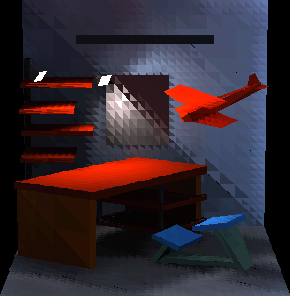
\includegraphics[width=.32\linewidth]{figures/radiosity}\label{fig:splash2:radiosity}}\hfill%
\subbottom[\theapp{raytrace}]{\centering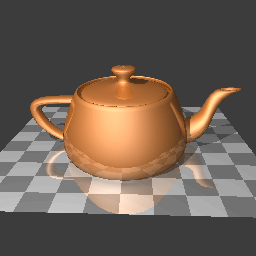
\includegraphics[width=.32\linewidth]{figures/raytrace}\label{fig:splash2:raytrace}}\hfill%
\subbottom[\theapp{volrend}]{\centering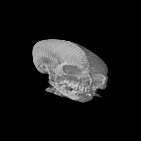
\includegraphics[width=.32\linewidth]{figures/volrend}\label{fig:splash2:volrend}}%
\caption{\SPLASH applications}%
\label{fig:splash2}%
\end{figure}

From the \SPLASH*~\cite{woo:splash2} benchmark set, we use three applications: \theapp{radiosity}, \theapp{raytrace}, and \theapp{volrend}.
Every application makes use of worker processes, which all do a part of the work.
Every \MicroBlaze runs exactly one of such a process.
Screen dumps of these applications are shown in \vref{fig:splash2}.
The applications are used in \cref{c:hardware,c:memory}.

\Theapp*{radiosity} splits a \ndim{3} model of a room into small triangles.
Then, the interaction of the luminance of all pairs of triangles is calculated, starting from the lamps, which illuminate the otherwise dark room.
Iteratively, all pairs are processed, until the distribution of light stabilizes.
The program exhibits chaotic memory accesses, which result in much synchronization and cache coherency traffic.
Drawing the output, as shown in \vref{fig:splash2:radiosity}, is not part of the benchmark itself, and is an optional step afterwards.
However, it shows an often-occurring bug: only the bottom-left part of the square in the middle is lit---the output is somewhat non-deterministic.

Next, \theapp*{raytrace} renders a teapot, including reflections.
The rendering is done in a single pass.
It splits the work in packets of 8$\times$8 pixels, which are distributed among all worker processes.
The default data type for all computations is a \lstinline|double|.
As the \MicroBlaze has only hardware support for \lstinline|float|s, this is a performance penalty.
Interestingly, when all \lstinline|double|s are replaced by \lstinline|float|s, the output is bit-by-bit identical, but the performance increases almost by a factor of four.
For all experiments, the original code with \lstinline|double|s is used.

Finally, \theapp*{volrend} draws a skull, based on a \ndim{3} model out of voxels.
Similar to \theapp{raytrace}, the rendering is split in packets of a fixed amount of output pixels, which are drawn concurrently.
The program shows an animation of a rotating skull.
%\todo{Possibly insert some statistics, profiling (prf snapshots).
%However, they depend on the hardware configuration, which is not fixed at this point.}

\subsection{\PARSEC}
\label{s:parsec}

From the \PARSEC* benchmark suite~\cite{bienia:benchmark_multiprocs}, only \theapp*{fluidanimate} is used.
This program does a particle simulation.
Similar to \theapp{radiosity}, the interactions between pairs of particles are calculated, which result in a chaotic memory access pattern.
This application is used in \cref{c:hardware}.

Of all other applications of the benchmark suite, only \theapp{blackscholes} is runnable.
However, it is of limited use, as it does not use synchronization between worker processes.
The other applications are not compilable, because of dependencies on libraries that are not portable to non-standard platforms such as a \MicroBlaze and \Starburst, or are not runnable, because of memory constraints.

\subsection{\NoFib}
\label{s:nofib}

In \cref{c:concurrency}, concurrency is evaluated using functional languages.
We implemented a functional language on top of Pthread for x86 systems and \Helix.
The details of the implementation are discussed in that specific chapter.
The applications we use are taken from the Haskell \NoFib*~\cite{nofib} benchmark suite.
For completeness, we briefly discuss the applications below.

\Theapp*{coins} counts the number of ways one can pay a specific amount of money, with a given set of coins.
\Theapp*{queens} determines in how many ways $n$ queens on an $n\times n$ chessboard can be placed, such that they cannot capture each other.
\Theapp*{parfib} calculates the Fibonacci number of a given point in the sequence in an inefficient, but parallel way.
\Theapp*{partak} is a parallel version of the recursive Tak function $\tau$, which is designed to have an unpredictable amount of remaining work in each step of the computation.
\Theapp*{prsa} encrypts a string of tokens using the \noac{RSA} algorithm.

%\ctable[caption={\textsc{Applications}},label={t:starburst:apps}]{llrS[table-format=5.0]}{
%	\tnote[a]{\footnotesize All other applications of the set are not runnable, because of dependency problems or memory requirements.}}{
%	\FL benchmark set					& application				& code size & {mutexes} \ML
%	\multirow{1}{*}{PARSEC\tmark[a]}	& \texttt{fluidanimate}		& \SI{494}{\Kilo\byte} & 4403 \ML
%	\multirow{3}{*}{SPLASH-2}			& \texttt{radiosity}		& \SI{261}{\Kilo\byte} & 26034 \NN
%										& \texttt{raytrace}			& \SI{244}{\Kilo\byte} & 35 \NN
%										& \texttt{volrend}			& \SI{421}{\Kilo\byte} & 37 \LL
%}

